\section{Déroulement du projet}
\label{sec:deroulement}

\paragraph{Chapeau} Dans cette section, nous décrivons comment le projet a été réalisé en équipe : la répartition des tâches, la synchronisation du travail entre membres de l'équipe, etc.

\subsection{Répartition des tâches}

\begin{center}
\begin{tabular} {|p{3cm}|p{3cm}|}
\hline
AYAD Ishak & METIDJI Fares\\
\hline
UAL & UAL\\
\hline
Banc de registre & Unité d'adressage\\
\hline
Unité de contrôle & \\
\hline
 Modifications personnelles & \\
\hline

\end{tabular}
\end{center}

\begin{center}
\def\angle{0}
\def\radius{3}
\def\cyclelist{{"orange","blue","red","green"}}
\newcount\cyclecount \cyclecount=-1
\newcount\ind \ind=-1
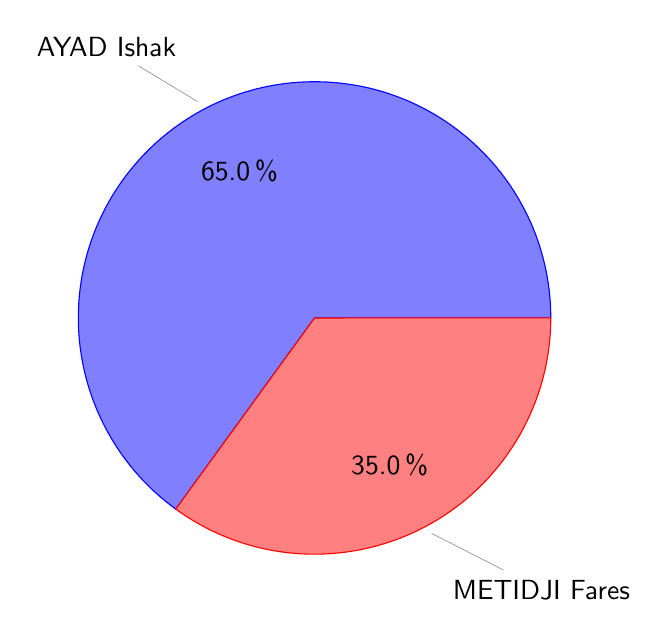
\begin{tikzpicture}[nodes = {font=\sffamily}]
  \foreach \percent/\name in {
      65.0/AYAD Ishak,
      35.0/METIDJI Fares,
    } {
      \ifx\percent\empty\else
        \global\advance\cyclecount by 1
        \global\advance\ind by 1
        \ifnum3<\cyclecount
          \global\cyclecount=0
          \global\ind=0
        \fi
        \pgfmathparse{\cyclelist[\the\ind]}
        \edef\color{\pgfmathresult}    
        \draw[fill={\color!50},draw={\color}] (0,0) -- (\angle:\radius)
          arc (\angle:\angle+\percent*3.6:\radius) -- cycle;
        \node at (\angle+0.5*\percent*3.6:0.7*\radius) {\percent\,\%};
        \node[pin=\angle+0.5*\percent*3.6:\name]
          at (\angle+0.5*\percent*3.6:\radius) {};
        \pgfmathparse{\angle+\percent*3.6} 
        \xdef\angle{\pgfmathresult}
        \angle
      \fi
    };
\end{tikzpicture}
\end{center}

\subsection{Synchronisation du travail}
\begin{itemize}
\item Pour la réalisation du projet nous avons utilisé le service web d'hébergement et de gestion de développement de logiciels GitHub pour synchroniser nos travaux.Ce dernier nous a permis d’effectuer des commites à un rythme élevé au commencement du projet pour que tous les membre de l'équipe aient accès aux bases ,puis après la répartition des tâches le rythme a diminué.
\item Pour la rédaction de ce document nous avons utilisé la plateforme web Overleaf pour répartir les taches, le rythme de rédaction a été très élevé à la fin du projet. 
\end{itemize}

\subsection{Problèmes rencontrés}
\begin{enumerate}
\item L’implémentation de l’opération soustraction.
\item Réalisation de l'unité d'adressage.
\item La compréhension de l'utilité d'un registre d'adresse de données.
\item La compréhension de certain signaux de sorties de l'UC (EXT).
\item notre Bascule D avait un problème donc nous avons utilisé le registre fourni par Logisim. 
\end{enumerate}

\clearpage
\subsection{Calendrier}

\fig{images/calen.PNG}{18cm}{9cm}{Calendrier}{calendrier}